\documentclass{article}
\usepackage{graphicx} % Required for inserting images
\usepackage{amsmath}
\usepackage{amssymb}

\title{DPD Smearing Function}
\author{Lars Nelson}
\date{June 2025}

\begin{document}

\maketitle

\section{Introduction}
This work is motivated by a desire to find a smearing function capable of reproducing the interaction potential between DPD particles in field-theoretic simulations.

\section{DPD Potential}
Interaction potential is not explicitly defined in DPD simulations; rather, particles within a critical radius \(r_c\) of each other exert a defined force on each other based on interaction parameter \(a_{ij}\):
\[F_{ij}^C(\mathbf{r_{ij}}) = a_{ij}\left(1-\frac{|\mathbf{r_{ij}}|}{r_c}\right)\mathbf{e_{ij}},\]
\noindent where \(\mathbf{e_{ij}, r_{ij}}\) are the unit and displacement vectors from particle \(i\) to particle \(j\). The potential can be recovered from the interaction force by taking advantage of spherical symmetry in the force vector's magnitude and direction:
\[\bar{u}_{DPD} (\mathbf{r}) = -\int^\mathbf{r}_\mathbf{r_c} F^C_{ij}(\mathbf{r}) \cdot d\mathbf{r} = -\int_{r_c}^r a_{ij}(1-r/r_c)dr\]
\begin{equation}
    \bar{u}_{DPD}= \begin{cases} a_{ij}\left(\frac{|\mathbf{r}|^2}{2r_c} - |\mathbf{r}| + \frac{r_c}{2}\right) & |\mathbf{r}| \leq r_c \\
    0 & |\mathbf{r}| > r_c
    \end{cases}\:.
    \label{eq:u_dpd}
\end{equation}

\section{Smearing Function}
In order to deal with ultraviolent divergences in field-theoretic simulations, it is beneficial to represent particles as ``smeared'' mass densities rather than as point particles. A total interaction potential \(\bar{U}\) arises from the structure of the smearing function \(\Gamma(\mathbf{r})\). With fine-tuning of this structure, this total interaction potential can be made equivalent to an effective potential \(\bar{u}_{eff}\) between two point particles. Since DPD simulations model beads as point particles, we wish to find a \(\Gamma({\mathbf{r}})\) such that \(\bar{u}_{eff}(\mathbf{r_0}-\mathbf{r'_0}) = \int d\mathbf{r}\int d\mathbf{r'} \; \Gamma(\mathbf{r}-\mathbf{r_0}) \bar{u}(\mathbf{r}-\mathbf{r'}) \Gamma(\mathbf{r'}-\mathbf{r'_0})\) is the DPD potential found in equation \ref{eq:u_dpd}. Note that \(\bar{u}(\mathbf{r}-\mathbf{r_0})\) here is the Dirac delta function, \(u_0\delta(\mathbf{r}-\mathbf{r_0})\), used for pairwise interactions in the Edwards model.

The calculation of the effective potential between two particles is equivalent to a convolution of the smearing function with itself:

\[\bar{u}_{eff}(\mathbf{r_0}-\mathbf{r'_0}) = \int d\mathbf{r}\int d\mathbf{r'} \; \Gamma(\mathbf{r}-\mathbf{r_0}) \bar{u}(\mathbf{r}-\mathbf{r'}) \Gamma(\mathbf{r'}-\mathbf{r'_0})\]
\[= \int d\mathbf{r}\int d\mathbf{r'} \; \Gamma(\mathbf{r}-\mathbf{r_0}) u_0 \delta(\mathbf{r}-\mathbf{r'}) \Gamma(\mathbf{r'}-\mathbf{r'_0})\]
\[= u_0 \int d\mathbf{r'} \;   \Gamma(\mathbf{r'}-\mathbf{r'_0}) \int d\mathbf{r} \; \delta(\mathbf{r}-\mathbf{r'})\Gamma(\mathbf{r}-\mathbf{r_0})\]
\[= u_0 \int d\mathbf{r'} \;   \Gamma(\mathbf{r'}-\mathbf{r'_0}) \int d(\mathbf{r}-\mathbf{r_0}) \; \delta(\mathbf{r}-\mathbf{r_0} -(\mathbf{r'} - \mathbf{r_0}))\Gamma(\mathbf{r}-\mathbf{r_0})\]
\[= u_0 \int d\mathbf{r'} \;   \Gamma(\mathbf{r'}-\mathbf{r'_0}) \Gamma(\mathbf{r}'-\mathbf{r_0})\]
\[= u_0 \int d(\mathbf{r'} - \mathbf{r'_0}) \;   \Gamma(\mathbf{r'}-\mathbf{r'_0}) \Gamma(\mathbf{r}'-\mathbf{r'_0} - (\mathbf{r_0} - \mathbf{r'_0}))\]
\[ = u_0 (\Gamma *\Gamma)(\mathbf{r_0} - \mathbf{r'_0}).\]

This allows us to take advantage of the fact that convolution becomes multiplication in the Fourier frequency space:
\[ \mathcal{F}\left[\frac {\bar{u}_{eff}}{u_0} \right] (k) = \hat{\Gamma}(k)^2 \]
\[\Gamma (r) = \mathcal{F}^{-1} \left[ \pm \sqrt{\mathcal{F}\left[\frac {\bar{u}_{eff}}{u_0} \right] (k)} \right].\]

\section{Calculations}
Let \(p = \bar{u}_{eff}/u_0\):

\[p = \frac{a_{ij}}{u_0} \left(\frac{|\mathbf{r}|^2}{2r_c} - |\mathbf{r}| + \frac{r_c}{2}\right), \: |\mathbf{r}| \leq r_c.\]

We define a nondimensional length scale of the system as \( \tilde r = r / r_c\) and define a dimensionless potential number \(Po = \frac{a_{ij}r_c}{2 u_0}\):
\[\tilde{p}(\tilde{r}) = Po (\tilde{r}^2 - 2\tilde{r} + 1)\]

Since \(\tilde{p}\) is spherically symmetrical, we can simplify the 3D Fourier transform to a one-dimensional integral by aligning the vector \(\mathbf{k}\) with the z-axis such that \(\mathbf{r \cdot k} = rk \cos{\theta}\). This allows us to express the transform using spherical Bessel functions:
\[\hat{p}(k) = \int_{ \mathbb{R}^3} p(\mathbf{r}) e^{-i \mathbf{r \cdot k}} d\mathbf{r}\]
\[= \int_0^\infty \int_0^{2\pi} \int_0^\pi p(r) e^{-i rk \cos{\theta}} r^2\sin{\theta} \; d\theta \; d\phi \; dr\]
\[= 4 \pi \int_0^\infty p(r) \frac{\sin{kr}}{kr} r^2 dr\]

We define a nondimensional length scale of the system as \( \tilde r = r / r_c\) and define a dimensionless potential number \(Po = \frac{a_{ij}r_c}{2 u_0}\):
\[\tilde{p}(\tilde{r}) = Po (\tilde{r}^2 - 2\tilde{r} + 1)\]

We also define a nondimensional wavenumber \(\tilde{k} = kr_c\), which allows us to express the transform nondimensionally.

\[\tilde{\hat{p}}(\tilde k) = 4 \pi \int_0^{r_c} p(r) \frac{\sin{kr}}{kr}r^2 dr = 4 \pi r_c^3 \int^1_0 \tilde p (\tilde{r}) \frac{\sin{\tilde{k}\tilde{r}}}{\tilde{k}\tilde{r}}\tilde{r}^2d\tilde{r}\]
\[= 4 \pi r_c^3 Po \int^1_0 \left[ \tilde{r}^2-2\tilde{r}+1 \right] \frac{\sin{\tilde{k}\tilde{r}}}{\tilde{k}\tilde{r}}\tilde{r}^2d\tilde{r}\]
\[= 8 \pi r_c^3Po \left( \frac{1}{2\tilde{k}} \int_0^1 \tilde{r}^3 \sin{(\tilde{k}\tilde{r})} d\tilde{r} - \frac{1}{\tilde{k}}\int_0^1 \tilde{r}^2 \sin{(\tilde{k}\tilde{r})} d\tilde{r} + \frac{1}{2\tilde{k}} \int_0^1 \tilde{r} \sin{(\tilde{k}\tilde{r})} d\tilde{r} \right)\]

\[\tilde{\hat{p}}(\tilde {k})= 8 \pi r_c^3 Po \left( \frac{1}{\tilde{k}^4}\cos{\tilde{k}} - \frac{3}{\tilde{k}^5} \sin{\tilde{k}} + \frac{2}{\tilde{k}^4} \right)\]

\begin{equation}
    \boxed{\tilde{\hat{\Gamma}}(\tilde {k})= \sqrt{8 \pi r_c^3 Po \left( \frac{1}{\tilde{k}^4}\cos{\tilde{k}} - \frac{3}{\tilde{k}^5} \sin{\tilde{k}} + \frac{2}{\tilde{k}^4} \right)}}
    \label{eq:transformed}
 \end{equation}

Since it is difficult to find an analytical solution to the inverse Fourier transform of this function, we solve numerically for the smearing function in physical space. The validity of our analytical solution is discussed in section \ref{sec:confirmation} below.

\section{Confirmation}
\label{sec:confirmation}
In order to confirm our candidate smearing function, we plotted the smearing function in physical space after subjecting equation \ref{eq:transformed} to the numerical inverse spherical Fourier transform \(\mathcal{F}^{-1}[f(k)](r) = \frac{1}{2\pi^2} \sum_{k_i = 0}^N f(k_i) \frac{\sin{k_ir}}{k_ir} \Delta k\). The shape of this function is compared with the original nondimensionalized DPD potential \(u_{eff}\) in Figure \ref{fig:check_plot}. It can also be seen in the figure that our solution of \(\Gamma (r)\) satisfies the condition \((\Gamma *\Gamma)(r) = u_{eff}(r)/u_0\). The autocorrelation of the smearing function, given in red, closely matches DPD potential.

The solution was also confirmed by performing a numerical transform both ways, beginning with \(u_{eff}\) and finding \(\Gamma(r) = \mathcal{F}^{-1} \left[ \pm \sqrt{\mathcal{F}\left[\frac {\bar{u}_{eff}}{u_0} \right] (k)} \right]\) numerically. The results of this are shown in Figure \ref{fig:check_plot}, and match the analytical solution.

\begin{figure}
    \centering
    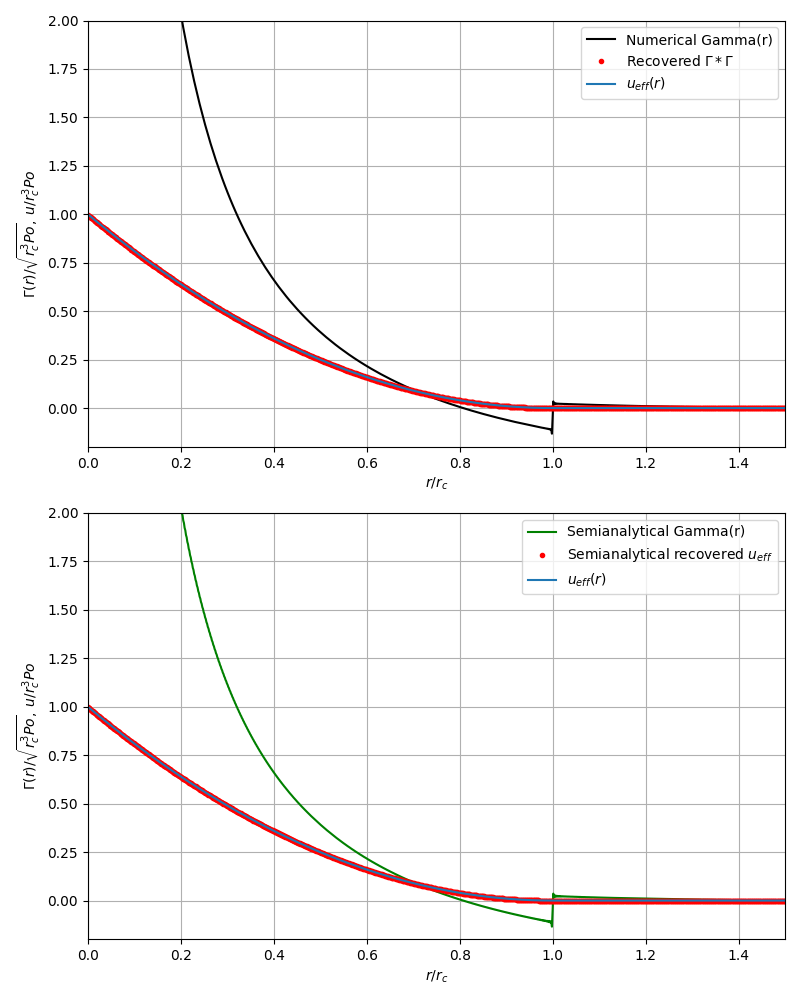
\includegraphics[width=0.95\linewidth]{check_fourier_transform.png}
    \caption{a) Comparison of smearing function as found numerically and the original effective DPD potential. b) Comparison of analytical solution of smearing function and DPD potential.}
    \label{fig:check_plot}
\end{figure}

\section{Discussion}
There are a few potentially concerning issues with the use of this solution as a smearing function for a point mass. These are as follows:
\begin{itemize}
    \item The value of \(\Gamma (r)\) increases very quickly as \(r\) approaches 0.
    \item The volume integral under the function does not equal unity.
    \item The smearing function drops below 0 in the range \(0.8 < \tilde r < 1.0\), signifying negative mass.
    \item The smearing function exhibits a quick jump with Gibbs phenomena at approximately \(\tilde r = 1\).
\end{itemize}

\subsection{Increase approaching \(\tilde r = 0\)}
A visual inspection of Figure \ref{fig:check_plot} shows that the value of \(\tilde \Gamma(\tilde r)\) increases quickly as \(\tilde r \to 0\). We find the limit of the function as follows:
\[\lim_{\tilde r \to 0} \tilde \Gamma (\tilde r) = \frac{1}{2 \pi^2 r_c^3} \lim_{\tilde r \to 0} \int_0^\infty \hat{\tilde \Gamma}(\tilde k) \frac{\sin \tilde k \tilde r}{\tilde k \tilde r} \tilde k^2 d \tilde k\]
\[ = \frac{1}{2 \pi^2 r_c^3} \int_0^\infty \hat{\tilde \Gamma}(\tilde k)  \tilde k^2 d \tilde k\]
\[ = \frac{1}{2 \pi^2 r_c^3} \int_0^\infty \sqrt{8 \pi r_c^3 Po \; \tilde k^4 \left( \frac{\cos \tilde k}{\tilde k^4} - \frac{3 \sin \tilde k}{\tilde k^5} + \frac{2}{\tilde k^4}\right)}  d\tilde k\]
\[ = \int_0^\infty \sqrt{\frac{2Po}{\pi^3 r_c^3} \left(\cos \tilde k - \frac{3 \sin \tilde k}{\tilde k} + 2\right)}  d\tilde k \: .\]
This integrand is nonzero and positive for all \(\tilde k \neq 0\); thus, the integral is positive infinite. This infinite limit at low radii could be problematic for numerical evaluation of potential, especially in systems where units are densely packed.

\subsection{Mass integral}
Since the smearing function represents a space distribution of a unit mass, we should expect the mass integral under the curve to be equal to 1:
\[ 4\pi \int_0^\infty \Gamma(r) r^2 dr = 1.\]
Without an analytical solution for \(\Gamma(r)\),  the integral must be computed numerically. This is quickly shown below:
\[M = 4\pi \int_0^\infty \Gamma(r) r^2dr = 4 \pi r_c^3 \int_0^\infty \tilde \Gamma (\tilde r) \tilde r^2 d \tilde r\]
\[\tilde \Gamma (\tilde r) = \frac{1}{2 \pi^2 r_c^3} \int_0^\infty \tilde{\hat{\Gamma}} (\tilde k) \frac{\sin \tilde k \tilde r}{\tilde k \tilde r} \tilde k^2 d\tilde k\]
\[M = \frac{2}{\pi} \int_0^\infty \int_0^\infty \tilde{\hat{\Gamma}} (\tilde k) \frac{\sin \tilde k \tilde r}{\tilde k \tilde r} \tilde k^2 \tilde r^2 d\tilde r d\tilde k\]
\[= \frac{2}{\pi} \int_0^\infty d\tilde k \: \tilde{\hat{\Gamma}}(\tilde k) \tilde k \int_0^1 \tilde r \sin \tilde k \tilde r d\tilde r\]
\[= \sqrt{\frac{32r_c^3Po}{\pi}} \int_0^\infty \sqrt{\left( \frac{\cos \tilde k}{\tilde k^4} - \frac{3 \sin \tilde k}{\tilde k^5} + \frac{2}{\tilde k^4} \right)} \left( \frac{\sin \tilde k - \tilde k \cos \tilde k}{\tilde k} \right) d\tilde k\]

The integrand simplifies to a square root of several periodic terms, each of which quickly trends to zero. In attempting to numerically determine the value of \(M\), it was determined that a factor of \(\sqrt{5}\) was required to bring the final mass integral to 1. It is unknown where this factor comes from.

The final, normalized smearing function is thus:
\[\tilde{\hat{\Gamma}}_{norm}(\tilde {k})= \frac{\sqrt{8 \pi r_c^3 Po \left( \frac{1}{\tilde{k}^4}\cos{\tilde{k}} - \frac{3}{\tilde{k}^5} \sin{\tilde{k}} + \frac{2}{\tilde{k}^4} \right)}}{\sqrt{\frac{32r_c^3Po}{5\pi}} \int_0^\infty \sqrt{\left( \frac{\cos \tilde k}{\tilde k^4} - \frac{3 \sin \tilde k}{\tilde k^5} + \frac{2}{\tilde k^4} \right)} \left( \frac{\sin \tilde k - \tilde k \cos \tilde k}{\tilde k} \right) d\tilde k}\]

\begin{equation}
    \boxed{\tilde{\hat{\Gamma}}_{norm}(\tilde {k})= \frac{\pi\sqrt{5}\sqrt{\left( \frac{1}{\tilde{k}^4}\cos{\tilde{k}} - \frac{3}{\tilde{k}^5} \sin{\tilde{k}} + \frac{2}{\tilde{k}^4} \right)}}{2 \int_0^\infty \sqrt{\left( \frac{\cos \tilde k}{\tilde k^4} - \frac{3 \sin \tilde k}{\tilde k^5} + \frac{2}{\tilde k^4} \right)} \left( \frac{\sin \tilde k - \tilde k \cos \tilde k}{\tilde k} \right) d\tilde k}}
    \label{eq:transformed}
 \end{equation}

 \textit{Note:} The normalization constant \(N = \sqrt{5} / M\) affects the effective potential \(u_{eff}(r) = \Gamma_{norm} * \Gamma_{norm}\). In order to restore the potential to the proper amplitude, we must factor the autocorrelation of \(\Gamma\) by \(M^2/5\).
 
\subsection{Negative mass}
As can be seen in Figure \ref{fig:check_plot}, the smearing function drops below 0 in the range \(0.8 < \tilde r < 1.0\), signifying negative mass. This is clearly nonphysical when the smearing function is considered as a mass distribution over space, and will have to be considered if we continue to implement the function in OpenFTS.

\subsection{Jump discontinuity at \(\tilde r = 1\)}
The jump at \(\tilde r = 1\) is likely caused by a discontinuity in the second derivative at the same point. The second derivative of the quadratic DPD potential is \(2 Po\) at all points lower than the critical radius; however, above the critical radius the function has a constant value of zero. This characteristic of the DPD potential allows for simpler modeling of molecules as particles, but causes problems for field simulations.

% Since \(p\) is spherically symmetrical, we can simplify the 3D Fourier transform to a one-dimensional integral by aligning the vector \(\mathbf{k}\) with the z-axis such that \(\mathbf{r \cdot k} = rk \cos{\theta}\). This allows us to express the transform using spherical Bessel functions:
% \[\hat{p}(k) = \int_{ \mathbb{R}^3} p(\mathbf{r}) e^{-i \mathbf{r \cdot k}} d\mathbf{r}\]
% \[= \int_0^\infty \int_0^{2\pi} \int_0^\pi p(r) e^{-i rk \cos{\theta}} r^2\sin{\theta} \; d\theta \; d\phi \; dr\]
% \[4 \pi \int_0^\infty p(r) \frac{\sin{kr}}{kr} r^2 dr\]
% \[ = 4 \pi \frac{a_{ij}}{u_0} \int_0^{r_c} \left[ \frac{r^2}{2r_c} -r + \frac{r_c}{2} \right] \frac{\sin{kr}}{kr}r^2dr\]
% \[= 4 \pi \frac{a_{ij}}{u_0} \left( \frac{1}{2r_ck} \int_0^{r_c} r^3 \sin{kr} dr - \frac{1}{k}\int_0^{r_c} r^2 \sin{kr} dr + \frac{r_c}{2k} \int_0^{r_c} r \sin{kr} dr \right)\]

% \begin{equation}
%     \boxed{\hat{p}(k)= 4 \pi \frac{a_{ij}}{u_0} \left( \frac{1}{k^4}\cos{kr_c} - \frac{3}{r_c k^5} \sin{kr_c} + \frac{2}{k^4} \right)}
%     \label{eq:transformed}
%  \end{equation}

\section{Conclusion}
The final, normalized smearing function for modeling DPD potential in field theoretic simulations is:
\begin{equation}
    \boxed{\tilde{\hat{\Gamma}}_{norm}(\tilde {k})= \frac{\pi\sqrt{5}\sqrt{\left( \frac{1}{\tilde{k}^4}\cos{\tilde{k}} - \frac{3}{\tilde{k}^5} \sin{\tilde{k}} + \frac{2}{\tilde{k}^4} \right)}}{2 \int_0^\infty \sqrt{\left( \frac{\cos \tilde k}{\tilde k^4} - \frac{3 \sin \tilde k}{\tilde k^5} + \frac{2}{\tilde k^4} \right)} \left( \frac{\sin \tilde k - \tilde k \cos \tilde k}{\tilde k} \right) d\tilde k}}
    \label{eq:transformed}
 \end{equation}

In order to ensure that the potential between two particles remains the same magnitude as in an analogous DPD simulation, the autocorrelation of the smearing function must be multiplied by a constant factor \(M^2 /5\), where

\[M = \sqrt{\frac{32r_c^3Po}{\pi}} \int_0^\infty \sqrt{\left( \frac{\cos \tilde k}{\tilde k^4} - \frac{3 \sin \tilde k}{\tilde k^5} + \frac{2}{\tilde k^4} \right)} \left( \frac{\sin \tilde k - \tilde k \cos \tilde k}{\tilde k} \right) d\tilde k\]

\end{document}

